\documentclass[lang=ngerman]{edoxarticle}


\newcommand{\vect}[3]{\begin{pmatrix} #1 \\ #2 \\ #3 \end{pmatrix}}
\renewcommand\examname{Klausur 1}
\renewcommand\pointsname{BE}

\begin{document}
\pdate{}
\begin{exam}{Mathematik Q2 GK}

\vskip20pt
{\LARGE\textbf{Vorblatt}}
\vskip20pt

Für die Bearbeitung der Aufgaben des Prüfungsteils A sind Zeichengeräte und ein
Wörterbuch zur deutschen Rechtschreibung zugelassen. Eine Verwendung von
weiteren Hilfsmitteln ist nicht zulässig.

Sie müssen den Prüfungsteil A \textbf{spätestens 35 Minuten} nach Prüfungsbeginn
abgeben. Die Hilfsmittel Taschenrechner und Formelsammlung erhalten Sie nach
Abgabe von Prüfungsteil A.

Sie müssen die \textbf{drei Pflichtaufgaben und zwei Wahlpflichtaufgaben} im
Prüfungsteil A bearbeiten.

\textbf{Tragen Sie die Aufgabennummern der zwei Wahlpflichtaufgaben ein, die
bewertet werden sollen.}

\vskip20pt
Wahlpflichtaufgabe Nr. \hbox to 4cm{\hrulefill}
\vskip10pt
Wahlpflichtaufgabe Nr. \hbox to 4cm{\hrulefill}
\vskip30pt
\textbf{Bestätigen Sie Ihre Entscheidung mit Ihrer Unterschrift.}
\vskip10pt
\hbox to \textwidth{Name, Vorname des Prüflings: \kern3.4cm\leaders\hrule\hfill}\vskip10pt
\hbox to \textwidth{Unterschrift des Prüflings: \kern4cm\leaders\hrule\hfill}

\newpage

\newpage
\wssection[AP]{Prüfungsteil A: Pflichtteil P}
\vskip10pt
\textbf{Bearbeiten Sie alle drei Aufgaben, eine Auswahl ist nicht vorgesehen.}
\vskip10pt
\exercise*[Aufgabe P1]{
Gegeben ist die Funktion $f$ mit $f(x)=3x^2+3x-6$.

\subexercise{
Zeigen Sie rechnerisch, dass $x=1$ und $x=-2$ die einzigen Nullstellen von $f$ sind.
\solve{
\[
3x^2+3x-6=0 \;|:3\; \Rightarrow\; x^2+x-2=0
\]
\[
x_{1,2}=-\frac12\pm\sqrt{\frac14+2}=-\frac12\pm\frac32
\]
\[
x_1=1,\qquad x_2=-2
\]
Da eine quadratische Gleichung höchstens zwei Lösungen besitzt, sind dies die einzigen Nullstellen.\pp[2]
}
}
\vskip8pt
\subexercise{
Berechnen Sie den Inhalt der Fläche, die die Funktion $f$ mit der $x$-Achse einschließt.
\solve{
Da die Parabel nach oben geöffnet ist und zwischen den Nullstellen unterhalb der $x$-Achse verläuft:
\[
A=-\int_{-2}^{1}\left(3x^2+3x-6\right)\,dx=-\left[x^3+\frac32x^2-6x\right]_{-2}^{1}
\]
\[
=-\left(\left(1+\frac32-6\right)-\left(-8+6+12\right)\right)=-\left(-\frac72-10\right)=\frac{27}{2}
\]
\[
A=\frac{27}{2}=13{,}5\ \text{FE}
\]
\pp[3]
}
}
}
\vskip8pt
\exercise*[Aufgabe P2]{
Gegeben ist die Ebene
\[
E:\;\vec x=\vect342+r\cdot\vect130+s\cdot\vect{-1}43.
\]
\subexercise{
Bestimmen Sie einen Normalenvektor der Ebene $E$ durch Ausprobieren mithilfe des Skalarprodukts. Der Normalenvektor ist senkrecht zu beiden Richtungsvektoren.

\emph{Hinweis: Wenn Sie keine Idee haben, nutzen Sie den Normalenvektor $\vect{4{,}5}{-1{,}5}{3{,}5}$.}
\solve{
Der gesuchte Normalenvektor $\vec n=\vect{n_1}{n_2}{n_3}$ steht senkrecht auf beiden Richtungsvektoren, das Skalarprodukt mit beiden ist also jeweils $0$:
\[
\vec n\cdot\vect130=0:\;\; n_1+3n_2=0 \qquad\qquad \vec n\cdot\vect{-1}43=0:\;\; -n_1+4n_2+3n_3=0
\]
Aus der ersten Gleichung: $n_1=-3n_2$. Eingesetzt in die zweite Gleichung:
\[
3n_2+4n_2+3n_3=0 \;\Longrightarrow\; 7n_2+3n_3=0
\]
Durch Ausprobieren: Mit $n_2=-3$ ergibt sich $n_3=7$ und damit $n_1=9$.
\[
\vec n=\vect9{-3}7
\]
\pp[2]
}
}
\vskip8pt
\subexercise{
Prüfen Sie, ob der Punkt $R(1|-2|0)$ auf der Ebene liegt.
\solve{
Gleichsetzen von Punkt und Ebenengleichung:
\[
\vect1{-2}0=\vect342+r\cdot\vect130+s\cdot\vect{-1}43
\]
liefert das Gleichungssystem
\[
\text{I:}\; 1=3+r-s \qquad \text{II:}\; -2=4+3r+4s \qquad \text{III:}\; 0=2+3s
\]
Aus III: $s=-\dfrac23$. Eingesetzt in I: $r=s-2=-\dfrac83$.

Probe in II: $3r+4s=3\cdot\left(-\dfrac83\right)+4\cdot\left(-\dfrac23\right)=-8-\dfrac83=-\dfrac{32}{3}\neq-6$.

Da Gleichung II nicht erfüllt ist, besitzt das System keine Lösung $(r,s)$. $R$ liegt \textbf{nicht} auf $E$.\pp[3]
}
}
}
\vskip8pt
\exercise*[Aufgabe P3]{
Untersuchen Sie, wie die Geraden $g$ und $h$ zueinander liegen. Berechnen Sie ggf. die Koordinaten des Schnittpunkts.
\[
g:\;\vec x=\vect314+r\cdot\vect1{-1}{-3};\qquad h:\;\vec x=\vect2{-1}6+s\cdot\vect{-3}39
\]
\subexercise{
Untersuchen Sie zunächst die Richtungsvektoren.
\solve{
\[
\vect{-3}39=-3\cdot\vect1{-1}{-3}
\]
Die Richtungsvektoren sind Vielfache voneinander -- $g$ und $h$ sind \textbf{parallel} (identisch oder echt parallel).\pp[2]
}
}
\vskip8pt
\subexercise{
Entscheiden Sie, ob $g$ und $h$ identisch oder echt parallel sind.
\solve{
Prüfen, ob der Stützpunkt von $h$, $(2|-1|6)$, auf $g$ liegt:
\[
\begin{array}{rll}
3+r=2 &\Rightarrow& r=-1\\
1-r=-1 &\Rightarrow& r=2\\
4-3r=6 &\Rightarrow& r=-\dfrac23
\end{array}
\]
Die Werte für $r$ stimmen nicht überein -- der Punkt liegt nicht auf $g$. Die Geraden sind also \textbf{echt parallel} und besitzen keinen Schnittpunkt.\pp[3]
}
}
}

\newpage
\wssection[AW]{Prüfungsteil A: Wahlpflichtteil W}
\vskip10pt
\textbf{Wählen Sie zwei der insgesamt vier Aufgaben aus und bearbeiten diese.}
\vskip10pt
\exercise*[Aufgabe W1]{
Gegeben ist die Funktion $g$ mit $g(x)=e^{-2x}+2x$. Berechnen Sie die Extrempunkte von $g$.
\solve{
\[
g'(x)=-2e^{-2x}+2
\]
Notwendige Bedingung: $g'(x)=0 \Rightarrow e^{-2x}=1 \Rightarrow x=0$.\pp[2]
\[
g''(x)=4e^{-2x},\qquad g''(0)=4>0 \;\Rightarrow\; \text{Tiefpunkt}
\]
\[
g(0)=1
\]
Tiefpunkt $\text{TP}(0|1)$.\pp[3]
}
}
\vskip8pt
\exercise*[Aufgabe W2]{
Gegeben ist die Funktion $f$ mit $f(x)=(3x^2+6)e^{-0{,}5x}$.

\subexercise{
Bestimmen Sie unter Anwendung der Ableitungsregeln die erste Ableitung von $f$.

\emph{Zur Kontrolle: $f'(x)=(-1{,}5x^2+6x-3)e^{-0{,}5x}$}
\solve{
Produktregel mit $u(x)=3x^2+6$, $v(x)=e^{-0{,}5x}$:
\[
f'(x)=6x\cdot e^{-0{,}5x}+(3x^2+6)\cdot(-0{,}5)e^{-0{,}5x}
\]
\[
f'(x)=\left(6x-1{,}5x^2-3\right)e^{-0{,}5x}=\left(-1{,}5x^2+6x-3\right)e^{-0{,}5x}
\]
\pp[3]
}
}
\vskip8pt
\subexercise{
Bestimmen Sie die Gleichung der Tangente an den Graphen von $f$ an der Stelle $x=0$.
\solve{
\[
f(0)=6,\qquad f'(0)=-3
\]
Tangente: $y=-3x+6$.\pp[2]
}
}
}
\vskip8pt
\exercise*[Aufgabe W3]{
Bestimmen Sie unter vollständiger Angabe des Lösungswegs die Lösung des linearen Gleichungssystems.
\[
\begin{array}{rcrcrcr}
\text{I}&&6x_1-2x_2+6x_3&=&-34\\
\text{II}&&2x_1-x_2-x_3&=&-8\\
\text{III}&&2x_1-2x_2+6x_3&=&-14
\end{array}
\]
\solve{
$\text{I}-3\cdot\text{II}$:
\[
6x_1-2x_2+6x_3-\left(6x_1-3x_2-3x_3\right)=-34-(-24)
\]
\[
x_2+9x_3=-10 \quad(\text{IV})
\]
\pp

$\text{I}-3\cdot\text{III}$:
\[
6x_1-2x_2+6x_3-\left(6x_1-6x_2+18x_3\right)=-34-(-42)
\]
\[
4x_2-12x_3=8 \quad\Rightarrow\quad x_2-3x_3=2 \quad(\text{V})
\]
\pp

$\text{IV}-\text{V}$: $12x_3=-12 \Rightarrow x_3=-1$.\pp

Einsetzen in (V): $x_2-3\cdot(-1)=2 \Rightarrow x_2=-1$.\pp

Einsetzen in I: $6x_1-2\cdot(-1)+6\cdot(-1)=-34 \Rightarrow 6x_1-4=-34 \Rightarrow x_1=-5$.\pp
\[
L=\{(-5;-1;-1)\}
\]
}
}
\vskip8pt
\exercise*[Aufgabe W4]{
Die Punkte $A(-4|3|2)$, $B(2|1|-5)$ und $C(5|3|-3)$ bilden das Dreieck $ABC$.

\subexercise{
Zeigen Sie, dass das Dreieck am Punkt $B$ einen rechten Winkel besitzt.
\solve{
\[
\overrightarrow{BA}=\vect{-6}27,\qquad \overrightarrow{BC}=\vect32{2}
\]
\[
\overrightarrow{BA}\cdot\overrightarrow{BC}=-18+4+14=0
\]
Da das Skalarprodukt $0$ ist, stehen $\overrightarrow{BA}$ und $\overrightarrow{BC}$ senkrecht aufeinander -- rechter Winkel bei $B$.\pp[2]
}
}
\vskip8pt
\subexercise{
Bestimmen Sie die Länge der Seite $AB$.
\solve{
\[
\left|\overrightarrow{AB}\right|=\sqrt{6^2+(-2)^2+(-7)^2}=\sqrt{36+4+49}=\sqrt{89}\approx9{,}43
\]
\pp
}
}
\vskip8pt
\subexercise{
Ermitteln Sie die Koordinaten eines Punktes $D$, sodass das Viereck $ABCD$ ein Rechteck ist.
\solve{
Da der rechte Winkel bei $B$ liegt, muss $D=A+\overrightarrow{BC}$ gelten:
\[
D=\vect{-4}32+\vect322=\vect{-1}{5}{4}
\]
\pp[2]
}
}
}

\newpage
\wssection[B]{Prüfungsteil B: Aufgaben mit Hilfsmitteln}
\vskip10pt
\exercise*[Aufgabe B1]{
Gegeben ist die Funktion $f$ mit
\[
f(x)=-0{,}25\cdot\left(x^2-10x-40\right)\cdot e^{-0{,}2x}.
\]
Die Abbildung zeigt den Graphen der Funktion.

\begin{center}
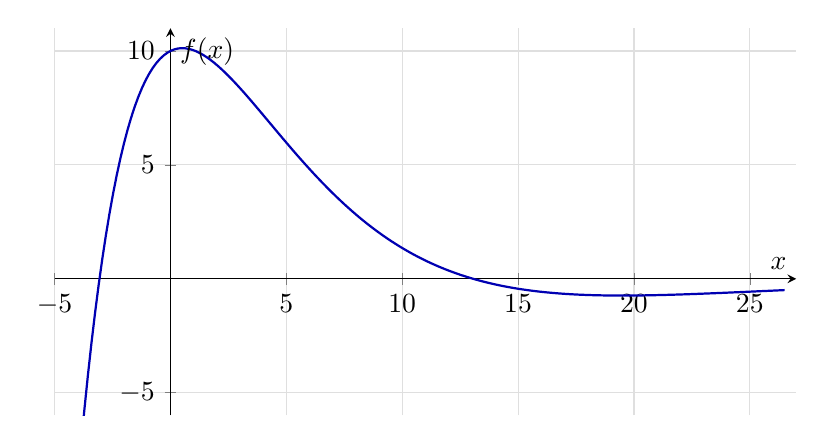
\begin{tikzpicture}
\begin{axis}[
  width=11cm, height=6.5cm,
  xmin=-5, xmax=27, ymin=-6, ymax=11,
  axis lines=middle, grid=both, grid style={gray!25},
  xlabel={$x$}, ylabel={$f(x)$},
  samples=200, domain=-4.5:26.5,
]
\addplot[thick, blue!70!black] {-0.25*(x^2-10*x-40)*exp(-0.2*x)};
\end{axis}
\end{tikzpicture}
\end{center}

\subexercise{
Geben Sie das Verhalten von $f$ im Unendlichen in mathematisch korrekter Schreibweise an.
\solve{
\[
\lim_{x\to\infty}f(x)=0,\qquad \lim_{x\to-\infty}f(x)=-\infty
\]
\pp[3]
}
}
\vskip8pt
\subexercise{
Bestimmen Sie rechnerisch die Koordinaten der Schnittpunkte von $f$ mit den Koordinatenachsen.
\solve{
$y$-Achse: $f(0)=-0{,}25\cdot(-40)\cdot1=10$, also $(0|10)$.\pp

$x$-Achse: $f(x)=0 \Leftrightarrow x^2-10x-40=0$ (da $e^{-0{,}2x}\neq0$):
\[
x_{1,2}=5\pm\sqrt{25+40}=5\pm\sqrt{65}
\]
\[
x_1\approx-3{,}06,\qquad x_2\approx13{,}06
\]
\pp[2]
}
}
\vskip8pt
\subexercise{
Bestimmen Sie alle Werte von $x$, für die gilt $f(x)=7$.
\solve{
Mit dem CAS-Rechner (transzendente Gleichung):
\[
x_1\approx-1{,}72,\qquad x_2\approx4{,}16
\]
\pp[3]
}
}
\vskip8pt
\subexercise{
Geben Sie die ersten drei Ableitungen von $f$ an.
\solve{
\[
f'(x)=\frac{1}{20}\left(x^2-20x+10\right)e^{-0{,}2x}
\]
\[
f''(x)=\frac{1}{100}\left(-x^2+30x-110\right)e^{-0{,}2x}
\]
\[
f'''(x)=\frac{1}{500}\left(x^2-40x+260\right)e^{-0{,}2x}
\]
\pp[3]
}
}
\vskip8pt
\subexercise{
Berechnen Sie die Extrempunkte von $f$.
\solve{
Notwendige Bedingung: $f'(x)=0 \Rightarrow x^2-20x+10=0 \Rightarrow x=10\pm3\sqrt{10}$.
\[
x_1\approx0{,}51,\qquad x_2\approx19{,}49
\]
\pp[3]

$f''(0{,}51)\approx-0{,}86<0 \Rightarrow$ Hochpunkt $\text{HP}(0{,}51|10{,}12)$.

$f''(19{,}49)\approx0{,}02>0 \Rightarrow$ Tiefpunkt $\text{TP}(19{,}49|-0{,}74)$.\pp[4]
}
}
\vskip8pt
\subexercise{
Bestimmen Sie rechnerisch die Wendepunkte von $f$.
\solve{
Notwendige Bedingung: $f''(x)=0 \Rightarrow -x^2+30x-110=0 \Rightarrow x=15\pm\sqrt{115}$.
\[
x_1\approx4{,}28,\qquad x_2\approx25{,}72
\]
\pp[3]

Da $f'''(x_1)\neq0$ und $f'''(x_2)\neq0$ liegen echte Wendepunkte vor:
\[
\text{W}_1(4{,}28|6{,}85),\qquad \text{W}_2(25{,}72|-0{,}53)
\]
\pp[3]
}
}
\vskip8pt
\subexercise{
Gegeben ist die Funktion $t$ mit $t(x)=-0{,}61x+7{,}44$. Zeigen Sie durch eine Rechnung, dass $t$ die Tangente an den Graphen von $f$ an der Stelle $x=10$ ist.
\solve{
\[
f(10)\approx1{,}35,\qquad f'(10)\approx-0{,}61
\]
Tangente durch $(10|f(10))$ mit Steigung $f'(10)$:
\[
y=-0{,}61(x-10)+1{,}35=-0{,}61x+7{,}44
\]
Das entspricht $t(x)$.\pp[4]
}
}
\vskip8pt
\subexercise{
(1) Zeigen Sie unter Anwendung der Ableitungsregeln, dass $F$ mit $F(x)=(1{,}25x^2-50)e^{-0{,}2x}$ eine Stammfunktion von $f$ ist.

(2) Berechnen Sie den Inhalt der Fläche, die der Graph von $f$ im ersten Quadranten mit der $y$-Achse und der $x$-Achse einschließt.
\solve{
(1) Produktregel:
\[
F'(x)=2{,}5x\cdot e^{-0{,}2x}+\left(1{,}25x^2-50\right)\cdot(-0{,}2)e^{-0{,}2x}
\]
\[
=\left(2{,}5x-0{,}25x^2+10\right)e^{-0{,}2x}=-0{,}25\left(x^2-10x-40\right)e^{-0{,}2x}=f(x)
\]
\pp[3]

(2) Die Fläche wird von $x=0$ bis zur positiven Nullstelle $x=5+\sqrt{65}$ begrenzt:
\[
A=F\left(5+\sqrt{65}\right)-F(0)\approx11{,}98-(-50)=61{,}98
\]
Die Fläche beträgt etwa $A\approx61{,}98$ FE.\pp[3]
}
}
\vskip8pt
\subexercise{
Die Punkte $A(0|0)$, $B(u|0)$, $C(0|f(u))$ und $D(u|f(u))$ bilden für $0<u<13$ die Eckpunkte eines Rechtecks $ABCD$.

(1) Skizzieren Sie das Rechteck für $u=6$ in obiger Abbildung.

(2) Der Wert von $u$ soll so gewählt werden, dass der Flächeninhalt des Rechtecks $ABCD$ maximal wird. Stellen Sie eine geeignete Funktion zur Ermittlung des gesuchten Werts auf und geben Sie mit Hilfe des CAS-Rechners den gesuchten Wert von $u$ sowie den zugehörigen Flächeninhalt $A$ an.
\solve{
(1) $f(6)\approx4{,}82$, das Rechteck reicht von $(0|0)$ bis $(6|4{,}82)$.\pp

(2) Flächenfunktion: $A(u)=u\cdot f(u)$.

Mit dem CAS-Rechner: $A'(u)=0$ für $u=5$ (im Intervall $0<u<13$).
\[
A(5)=5\cdot f(5)\approx29{,}89
\]
Der Flächeninhalt wird für $u=5$ mit $A\approx29{,}89$ FE maximal.\pp[4]
}
}
}

\newpage
\exercise*[Aufgabe B2]{
Die Abbildung zeigt ein Prisma mit den Eckpunkten $A(3|4|-1)$, $B(3|8|-1)$, $C$, $D$, $E(0|4|1)$ und $F(0|4|-1)$. Die Punkte $G(0|8|0)$ und $H(1{,}5|8|-1)$ sind die Mittelpunkte der Seiten $CD$ bzw.\ $BC$.

\begin{center}
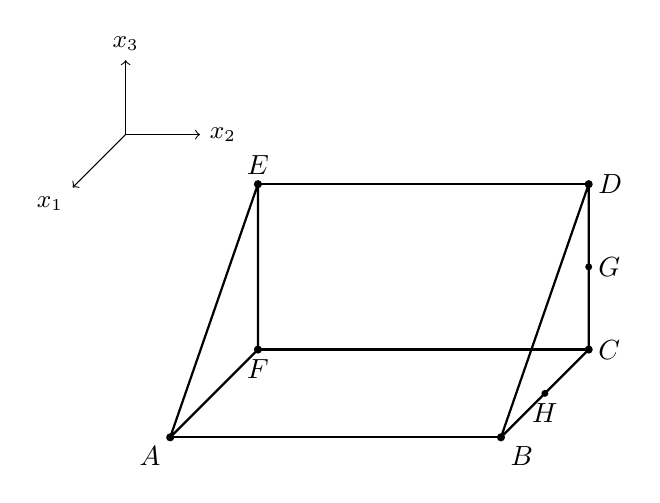
\begin{tikzpicture}[scale=1.05, line join=round]
\coordinate (A) at (2.939,-2.061);
\coordinate (B) at (6.939,-2.061);
\coordinate (C) at (8,-1);
\coordinate (D) at (8,1);
\coordinate (E) at (4,1);
\coordinate (F) at (4,-1);
\coordinate (G) at (8,0);
\coordinate (H) at (7.47,-1.53);
\coordinate (O) at (2.4,1.6);

\draw[thick] (A) -- (F) -- (E) -- cycle;
\draw[thick] (B) -- (C) -- (D) -- cycle;
\draw[thick] (A) -- (B);
\draw[thick] (F) -- (C);
\draw[thick] (E) -- (D);

\draw[->] (O) -- ++(-0.64,-0.64) node[below left]{\small$x_1$};
\draw[->] (O) -- ++(0.9,0) node[right]{\small$x_2$};
\draw[->] (O) -- ++(0,0.9) node[above]{\small$x_3$};

\fill (A) circle (1.4pt) node[below left]{$A$};
\fill (B) circle (1.4pt) node[below right]{$B$};
\fill (C) circle (1.4pt) node[right]{$C$};
\fill (D) circle (1.4pt) node[right]{$D$};
\fill (E) circle (1.4pt) node[above]{$E$};
\fill (F) circle (1.4pt) node[below]{$F$};
\fill (G) circle (1.2pt) node[right]{$G$};
\fill (H) circle (1.2pt) node[below]{$H$};
\end{tikzpicture}
\end{center}

\subexercise{
Geben Sie die Koordinaten der Punkte $C$ und $D$ an.
\solve{
$H$ ist Mittelpunkt von $BC$: $C=2H-B=\vect3{16}{-2}-\vect38{-1}=\vect0{8}{-1}$.\pp

$G$ ist Mittelpunkt von $CD$: $D=2G-C=\vect0{16}{0}-\vect08{-1}=\vect08{1}$.\pp
}
}
\vskip8pt
\subexercise{
(1) Weisen Sie durch eine Rechnung nach, dass die Fläche $ABCF$ ein Rechteck ist.

(2) Bestimmen Sie den Flächeninhalt des Rechtecks $ABCF$.
\solve{
(1)
\[
\overrightarrow{AB}=\vect040,\qquad \overrightarrow{AF}=\vect{-3}00,\qquad \overrightarrow{BC}=\vect{-3}00
\]
\[
\overrightarrow{AB}\cdot\overrightarrow{AF}=0,\qquad \overrightarrow{BC}=\overrightarrow{AF}
\]
$\overrightarrow{AB}\perp\overrightarrow{AF}$ und $\overrightarrow{BC}=\overrightarrow{AF}$: $ABCF$ ist ein Rechteck.\pp[3]

(2)
\[
A=\left|\overrightarrow{AB}\right|\cdot\left|\overrightarrow{AF}\right|=4\cdot3=12\ \text{FE}
\]
\pp[2]
}
}
\vskip8pt
\subexercise{
Berechnen Sie die Innenwinkel des Dreiecks $AFE$.
\solve{
\[
\overrightarrow{FA}=\vect300,\qquad \overrightarrow{FE}=\vect002,\qquad \overrightarrow{AE}=\vect{-3}02
\]
\[
\overrightarrow{FA}\cdot\overrightarrow{FE}=0 \;\Rightarrow\; \text{Winkel bei }F=90^\circ
\]
\[
\cos(\alpha)=\frac{\overrightarrow{AF}\cdot\overrightarrow{AE}}{|\overrightarrow{AF}||\overrightarrow{AE}|}=\frac{9}{3\cdot\sqrt{13}} \;\Rightarrow\; \alpha\approx33{,}69^\circ \text{ (bei }A\text{)}
\]
\[
\text{Winkel bei }E=180^\circ-90^\circ-33{,}69^\circ\approx56{,}31^\circ
\]
\pp[3]
}
}

\begin{center}
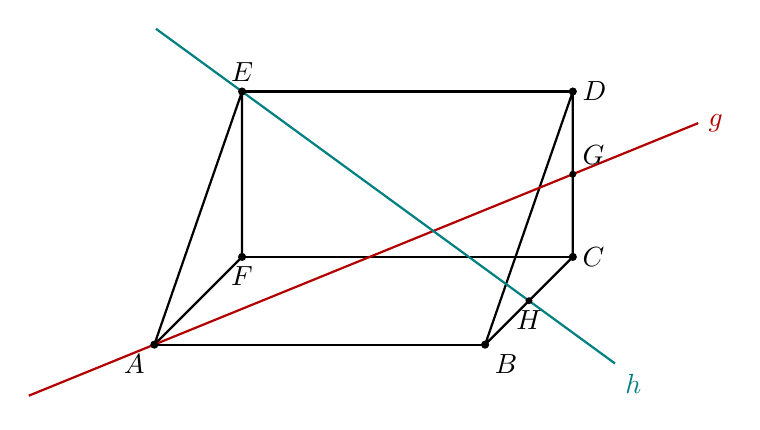
\begin{tikzpicture}[scale=1.05, line join=round]
\coordinate (A) at (2.939,-2.061);
\coordinate (B) at (6.939,-2.061);
\coordinate (C) at (8,-1);
\coordinate (D) at (8,1);
\coordinate (E) at (4,1);
\coordinate (F) at (4,-1);
\coordinate (G) at (8,0);
\coordinate (H) at (7.47,-1.53);

\draw[thick] (A) -- (F) -- (E) -- cycle;
\draw[thick] (B) -- (C) -- (D) -- cycle;
\draw[thick] (A) -- (B);
\draw[thick] (F) -- (C);
\draw[thick] (E) -- (D);

\draw[thick, red!70!black] (1.421,-2.679) -- (9.518,0.618) node[right]{$g$};
\draw[thick, teal] (2.959,1.759) -- (8.511,-2.289) node[below right]{$h$};

\fill (A) circle (1.4pt) node[below left]{$A$};
\fill (B) circle (1.4pt) node[below right]{$B$};
\fill (C) circle (1.4pt) node[right]{$C$};
\fill (D) circle (1.4pt) node[right]{$D$};
\fill (E) circle (1.4pt) node[above]{$E$};
\fill (F) circle (1.4pt) node[below]{$F$};
\fill (G) circle (1.2pt) node[above right]{$G$};
\fill (H) circle (1.2pt) node[below]{$H$};
\end{tikzpicture}
\end{center}
\vskip8pt
\subexercise{
Die Gerade $h$ verläuft durch die Punkte $E$ und $H$.

(1) Bestimmen Sie unter vollständiger Angabe des Lösungswegs eine Gleichung der Geraden $h$.

\emph{Hinweis: Wenn Sie die Geradengleichung nicht aufstellen können, verwenden Sie im Folgenden die Gleichung $h:\;\vec x=\vect{-1{,}5}03+r\cdot\vect{-3}{-8}4$.}

(2) Prüfen Sie durch eine Rechnung, ob der Punkt $R(-3|-4|5)$ auf der Geraden $h$ liegt.
\solve{
(1)
\[
\overrightarrow{EH}=H-E=\vect{1{,}5}{4}{-2}
\]
\[
h:\;\vec x=\vect041+r\cdot\vect{1{,}5}4{-2}
\]
\pp[3]

(2)
\[
\vect041+r\cdot\vect{1{,}5}4{-2}=\vect{-3}{-4}5 \;\Rightarrow\; r=-2 \text{ (in allen drei Zeilen konsistent)}
\]
$R$ liegt auf $h$.\pp[2]
}
}
\vskip8pt
\subexercise{
Die Gerade $g:\;\vec x=\vect34{-1}+r\cdot\vect{-1{,}5}{2}{0{,}5}$ geht durch die Punkte $A$ und $G$. Untersuchen Sie rechnerisch, welche Lage die Geraden $g$ und $h$ zueinander haben. Berechnen Sie ggf.\ den Schnittpunkt und Schnittwinkel.
\solve{
Die Richtungsvektoren sind nicht parallel (kein Vielfaches). Gleichsetzen:
\[
\vect34{-1}+r\cdot\vect{-1{,}5}2{0{,}5}=\vect041+s\cdot\vect{1{,}5}4{-2}
\]
liefert $r=\frac43$, $s=\frac23$ (in allen drei Gleichungen konsistent).\pp[3]

Die Geraden schneiden sich in
\[
\vect34{-1}+\frac43\cdot\vect{-1{,}5}2{0{,}5}=\vect{1}{\frac{20}{3}}{-\frac13}.
\]
\pp[2]

Schnittwinkel über die Richtungsvektoren $\vec u=\vect{-1{,}5}2{0{,}5}$ und $\vec v=\vect{1{,}5}4{-2}$:
\[
\cos\varphi=\frac{|\vec u\cdot\vec v|}{|\vec u|\cdot|\vec v|}=\frac{|-2{,}25+8-1|}{\sqrt{6{,}5}\cdot\sqrt{22{,}25}}=\frac{4{,}75}{\sqrt{144{,}625}}\approx0{,}395
\]
\[
\varphi\approx66{,}74^\circ
\]
\pp[2]
}
}
\vskip8pt
\subexercise{
Die Punkte $A$, $F$ und $E$ liegen in der Ebene $E_1$ und die Punkte $A$, $B$, $D$ und $E$ liegen in der Ebene $E_2$.

(1) Bestimmen Sie unter vollständiger Angabe des Lösungswegs eine Parametergleichung der Ebene $E_1$.

\emph{Hinweis: Wenn Sie die Gleichung nicht aufstellen können, verwenden Sie im Folgenden die Gleichung $E_1:\;\vec x=\vect{-3}41+r\cdot\vect{-6}02+s\cdot\vect{1{,}5}01$.}

Gegeben sind der Punkt $S(3|2|1)$ und die Gerade $k:\;\vec x=\vect040+t\cdot\vect{1{,}5}20$.

(2) Prüfen Sie durch eine Rechnung, ob der Punkt $S$ auf der Ebene $E_1$ liegt.

(3) Bestimmen Sie den Schnittwinkel zwischen der Geraden $k$ und der Ebene $E_1$.

(4) Untersuchen Sie mit Hilfe einer Rechnung, ob die Gerade $k$ die Ebene $E_1$ schneidet. Geben Sie ggf.\ den Schnittpunkt an.
\solve{
(1) $E_1$ durch $A,F,E$: $\overrightarrow{AF}=\vect{-3}00$, $\overrightarrow{AE}=\vect{-3}02$.
\[
E_1:\;\vec x=\vect34{-1}+r\cdot\vect{-3}00+s\cdot\vect{-3}02
\]
Für später nützlich, ein Normalenvektor: $\overrightarrow{AF}\times\overrightarrow{AE}=\vect060$, kurz $\vec n=\vect010$.\pp[3]

(2) Punktprobe über den Normalenvektor: $\overrightarrow{AS}=\vect0{-2}2$.
\[
\overrightarrow{AS}\cdot\vec n=0\cdot0+(-2)\cdot1+2\cdot0=-2\neq0
\]
Also $S\notin E_1$.\pp[2]

(3) Für den Schnittwinkel wird der Richtungsvektor $\vec u=\vect{1{,}5}20$ von $k$ benötigt:
\[
\sin\varphi=\frac{|\vec n\cdot\vec u|}{|\vec n|\cdot|\vec u|}=\frac{|0\cdot1{,}5+1\cdot2+0\cdot0|}{1\cdot\sqrt{1{,}5^2+2^2}}=\frac{2}{2{,}5}=0{,}8
\]
\[
\varphi=\arcsin(0{,}8)\approx53{,}13^\circ
\]
\pp[3]

(4) Da $\varphi\neq0^\circ$, ist $k$ nicht parallel zu $E_1$ -- die Gerade schneidet die Ebene in genau einem Punkt. Gleichsetzen:
\[
\vect040+t\cdot\vect{1{,}5}20=\vect34{-1}+r\cdot\vect{-3}00+s\cdot\vect{-3}02
\]
liefert aus der zweiten Gleichung $4+2t=4 \Rightarrow t=0$, aus der dritten $2s=1 \Rightarrow s=0{,}5$ und damit aus der ersten $r=0{,}5$ (Probe: alle drei Gleichungen konsistent).
\[
\vec x=\vect040
\]
Die Gerade $k$ schneidet $E_1$ im Punkt $(0|4|0)$.\pp[5]
}
}
}

\vskip20pt
\textbf{Zugelassene Hilfsmittel für Prüfungsteil B:}
\begin{itemize}
\item CAS-Taschenrechner
\item Formelsammlung
\item Wörterbuch zur deutschen Rechtschreibung
\end{itemize}

\setpoints{100}
\end{exam}
\end{document}